\begin{minipage}{0.75\linewidth}
\begin{figure}[h]
    \centering
    \begin{adjustbox}{max width=1.0\linewidth, keepaspectratio}
        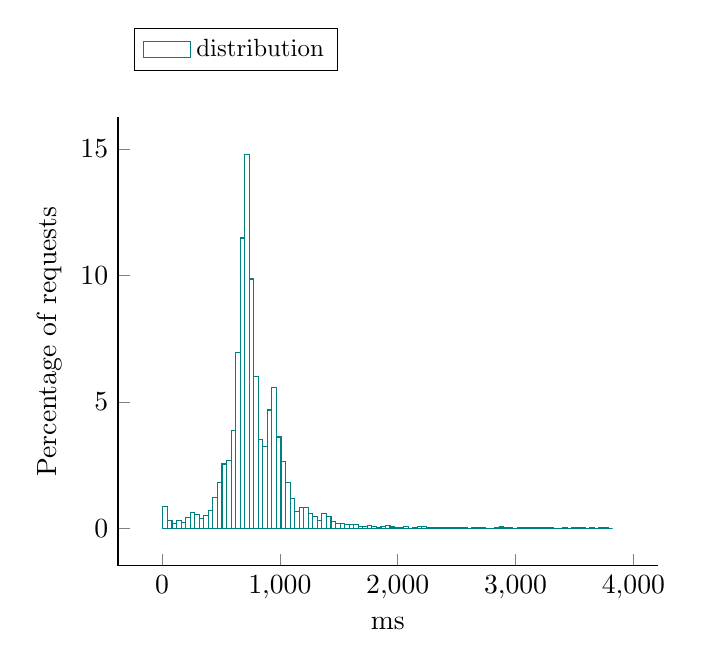
\begin{tikzpicture}
            \begin{axis}[ylabel = Percentage of requests, 
xlabel = ms, 
legend style = {nodes={scale=0.9, transform shape}, at={(0.03,1.2)}, anchor=north west, draw=black, fill=white, align=left, legend columns=3},
area style, mark size = 0pt,
 cycle list name = exotic,
  axis lines* = left]
		\addplot +[ybar interval] coordinates {
			 (8, 0.86811)
			 (46.54, 0.313775)
			 (85.08, 0.198724)
			 (123.62, 0.303316)
			 (162.16, 0.240561)
			 (200.7, 0.428825)
			 (239.24, 0.61709)
			 (277.78, 0.543876)
			 (316.32, 0.37653)
			 (354.86, 0.50204)
			 (393.4, 0.700764)
			 (431.94, 1.21326)
			 (470.48, 1.80943)
			 (509.02, 2.54158)
			 (547.56, 2.688)
			 (586.1, 3.88035)
			 (624.64, 6.94488)
			 (663.18, 11.4737)
			 (701.72, 14.7683)
			 (740.26, 9.85253)
			 (778.8, 6.01402)
			 (817.34, 3.49336)
			 (855.88, 3.22142)
			 (894.42, 4.67524)
			 (932.96, 5.56427)
			 (971.5, 3.60841)
			 (1010.04, 2.62525)
			 (1048.58, 1.81989)
			 (1087.12, 1.19234)
			 (1125.66, 0.648468)
			 (1164.2, 0.826273)
			 (1202.74, 0.805355)
			 (1241.28, 0.596172)
			 (1279.82, 0.470662)
			 (1318.36, 0.303316)
			 (1356.9, 0.575254)
			 (1395.44, 0.470662)
			 (1433.98, 0.261479)
			 (1472.52, 0.198724)
			 (1511.06, 0.198724)
			 (1549.6, 0.156887)
			 (1588.14, 0.135969)
			 (1626.68, 0.146428)
			 (1665.22, 0.0627549)
			 (1703.76, 0.0836733)
			 (1742.3, 0.12551)
			 (1780.84, 0.0732141)
			 (1819.38, 0.0418366)
			 (1857.92, 0.0836733)
			 (1896.46, 0.0941324)
			 (1935, 0.0522958)
			 (1973.54, 0.0104592)
			 (2012.08, 0.0313775)
			 (2050.62, 0.0732141)
			 (2089.16, 0)
			 (2127.7, 0.0209183)
			 (2166.24, 0.0627549)
			 (2204.78, 0.0732141)
			 (2243.32, 0.0104592)
			 (2281.86, 0.0104592)
			 (2320.4, 0.0209183)
			 (2358.94, 0.0418366)
			 (2397.48, 0.0313775)
			 (2436.02, 0.0418366)
			 (2474.56, 0.0209183)
			 (2513.1, 0.0418366)
			 (2551.64, 0.0209183)
			 (2590.18, 0)
			 (2628.72, 0.0104592)
			 (2667.26, 0.0313775)
			 (2705.8, 0.0313775)
			 (2744.34, 0)
			 (2782.88, 0)
			 (2821.42, 0.0209183)
			 (2859.96, 0.0522958)
			 (2898.5, 0.0209183)
			 (2937.04, 0.0418366)
			 (2975.58, 0)
			 (3014.12, 0.0418366)
			 (3052.66, 0.0313775)
			 (3091.2, 0.0313775)
			 (3129.74, 0.0104592)
			 (3168.28, 0.0418366)
			 (3206.82, 0.0209183)
			 (3245.36, 0.0104592)
			 (3283.9, 0.0313775)
			 (3322.44, 0)
			 (3360.98, 0)
			 (3399.52, 0.0209183)
			 (3438.06, 0)
			 (3476.6, 0.0209183)
			 (3515.14, 0.0313775)
			 (3553.68, 0.0313775)
			 (3592.22, 0)
			 (3630.76, 0.0104592)
			 (3669.3, 0)
			 (3707.84, 0.0104592)
			 (3746.38, 0.0209183)
			 (3784.92, 0)
			 (3823.46, 0.0104592)
		};
\addlegendentry{distribution};
           \end{axis}
      \end{tikzpicture}
  \end{adjustbox}
  \caption{Response time distribution - req = ReadUser-1}
\end{figure}
\end{minipage}\hfill\begin{minipage}{0.18\linewidth}
\begin{table}[h]
\begin{tabular}{|cc|}
\hline
\textbf{} & \textbf{ms}\\ \hline
 \Xhline{0.005\arrayrulewidth}
min & 8\\
 \Xhline{0.005\arrayrulewidth}
max & 3862\\
 \Xhline{0.005\arrayrulewidth}
mean & 796\\
 \Xhline{0.005\arrayrulewidth}
std & 324\\
\hline
\hline
 \Xhline{0.005\arrayrulewidth}
25th & 667\\
 \Xhline{0.005\arrayrulewidth}
50th & 739\\
 \Xhline{0.005\arrayrulewidth}
75th & 912\\
 \Xhline{0.005\arrayrulewidth}
80th & 946\\
 \Xhline{0.005\arrayrulewidth}
85th & 987\\
 \Xhline{0.005\arrayrulewidth}
90th & 1059\\
 \Xhline{0.005\arrayrulewidth}
95th & 1253\\
 \Xhline{0.005\arrayrulewidth}
99th & 2110\\
\hline
\end{tabular}
\caption{Response time}
\end{table}
\end{minipage}\hfill